\documentclass{beamer}
\usepackage[utf8]{inputenc}
\usepackage{amssymb}
\usepackage{amsmath}
\usepackage{dsfont}
\usepackage{stmaryrd}
\usepackage{graphicx}
\usepackage{listings}
\RequirePackage{tikz}
\usetikzlibrary{arrows}

%\usepackage{animate}
%\usepackage{multimedia}
\usepackage{hyperref}
\usepackage{media9}

\lstset{language=C++,
  basicstyle=\tiny,
  frame=single,
  captionpos=b,
  linewidth=1.02\linewidth,
  commentstyle=\color{green},
  stringstyle=\color{red},
  identifierstyle=\ttfamily,
  keywordstyle=\color{blue},
  texcl=true
%  breaklines=true
}
\newcommand{\patternscale}{.3}
\newcommand{\patternspace}{1mm}
\graphicspath{{./images/}{./images/video/}}
\addmediapath{./images/video/}

\title{Optimisation stochastique, (RJ)MCMC\\ et applications g\'eospatiales}
\author{\underline{Mathieu Brédif}, \underline{Julien Perret}, Bahman Soheilian\\Mickael Brasebin et Alexandre Hervieu}
\institute{IGN}
\date{2015}

\begin{document}
\frame{\titlepage}
 
 
\section{Introduction}

\begin{frame}
\frametitle{Contexte}
TODO: JP
\begin{itemize}
\item La recherche de l'IGN a souvent des probl\`emes d'optimisation (comme tout le monde)
\item D\'eveloppement d'outils \emph{sp\'ecifiques} (g\'en\'eralisation carto)
\item D\'eveloppement d'une biblioth\`eque plus \emph{g\'en\'erique}
\end{itemize}
\end{frame}


\begin{frame}
\frametitle{RJMCMC et MPP}
TODO: MB
rappel vite fait, notations, noyaux...
\end{frame}



\section{Applications}

\begin{frame}
TODO: MB
images resultats
\end{frame}

\begin{frame}
\frametitle{Reconstruction d'emprises de bâtiments rectangulaires}
\emph{Le probl\`eme~:} 
\begin{itemize}
\item Détecter des emprises de bâtiments sur un MNS satellite.
\end{itemize}
\emph{Les concepts~:}
\begin{itemize}
\item MPP~:  $\mathcal{C} = \cup_{n}\mathcal{B}^n$\\
avec $\mathcal{B}=[0,W]\times[0,H]\times[-S,S]^2\times[1/R,R] \subset  \mathds{R}^{5}$
\item Noyaux~: Naissance/mort, translation d'une arête, rotation/homothétie autour d'un coin, Division/Fusion
\item Processus de référence~:
\begin{itemize}
\item Processus de poisson sur $n$
\item Uniforme sur $\mathcal{B}$
\end{itemize}
\item \'Energie~: $E = \sum_i E_1(x_i) + \sum_{i<j} E_2(x_i,x_j)$
\begin{itemize}
\item $E_1(x_i)=\alpha_{0} - E_{data}(x_i)$ avec $\alpha_{0}>0$ ;
\item $E_2(x_i,x_j) = surface(x_i \cap x_j)$.
\end{itemize}
\end{itemize}
\end{frame}


\begin{frame}
\frametitle{Simplu3D}
\emph{Le probl\`eme~:}  Simulation des droits \`a batir
\begin{itemize}
\item Génération de configurations bâties pour évaluer l'influence des réglements des PLU
\end{itemize}
\emph{Les concepts~:}
\begin{columns}
\begin{column}{0.55\textwidth}
\begin{itemize}
\item MPP~:  $ \mathcal{C} =\mathcal{PLU} \cap \cup_{n} \mathcal{B}^n$  avec $\mathcal{B}  \subset  \mathds{R}^{6}$
\item Noyaux~: mêmes noyaux + Changement de hauteur
\end{itemize}
\end{column}
\begin{column}{0.45\textwidth}
 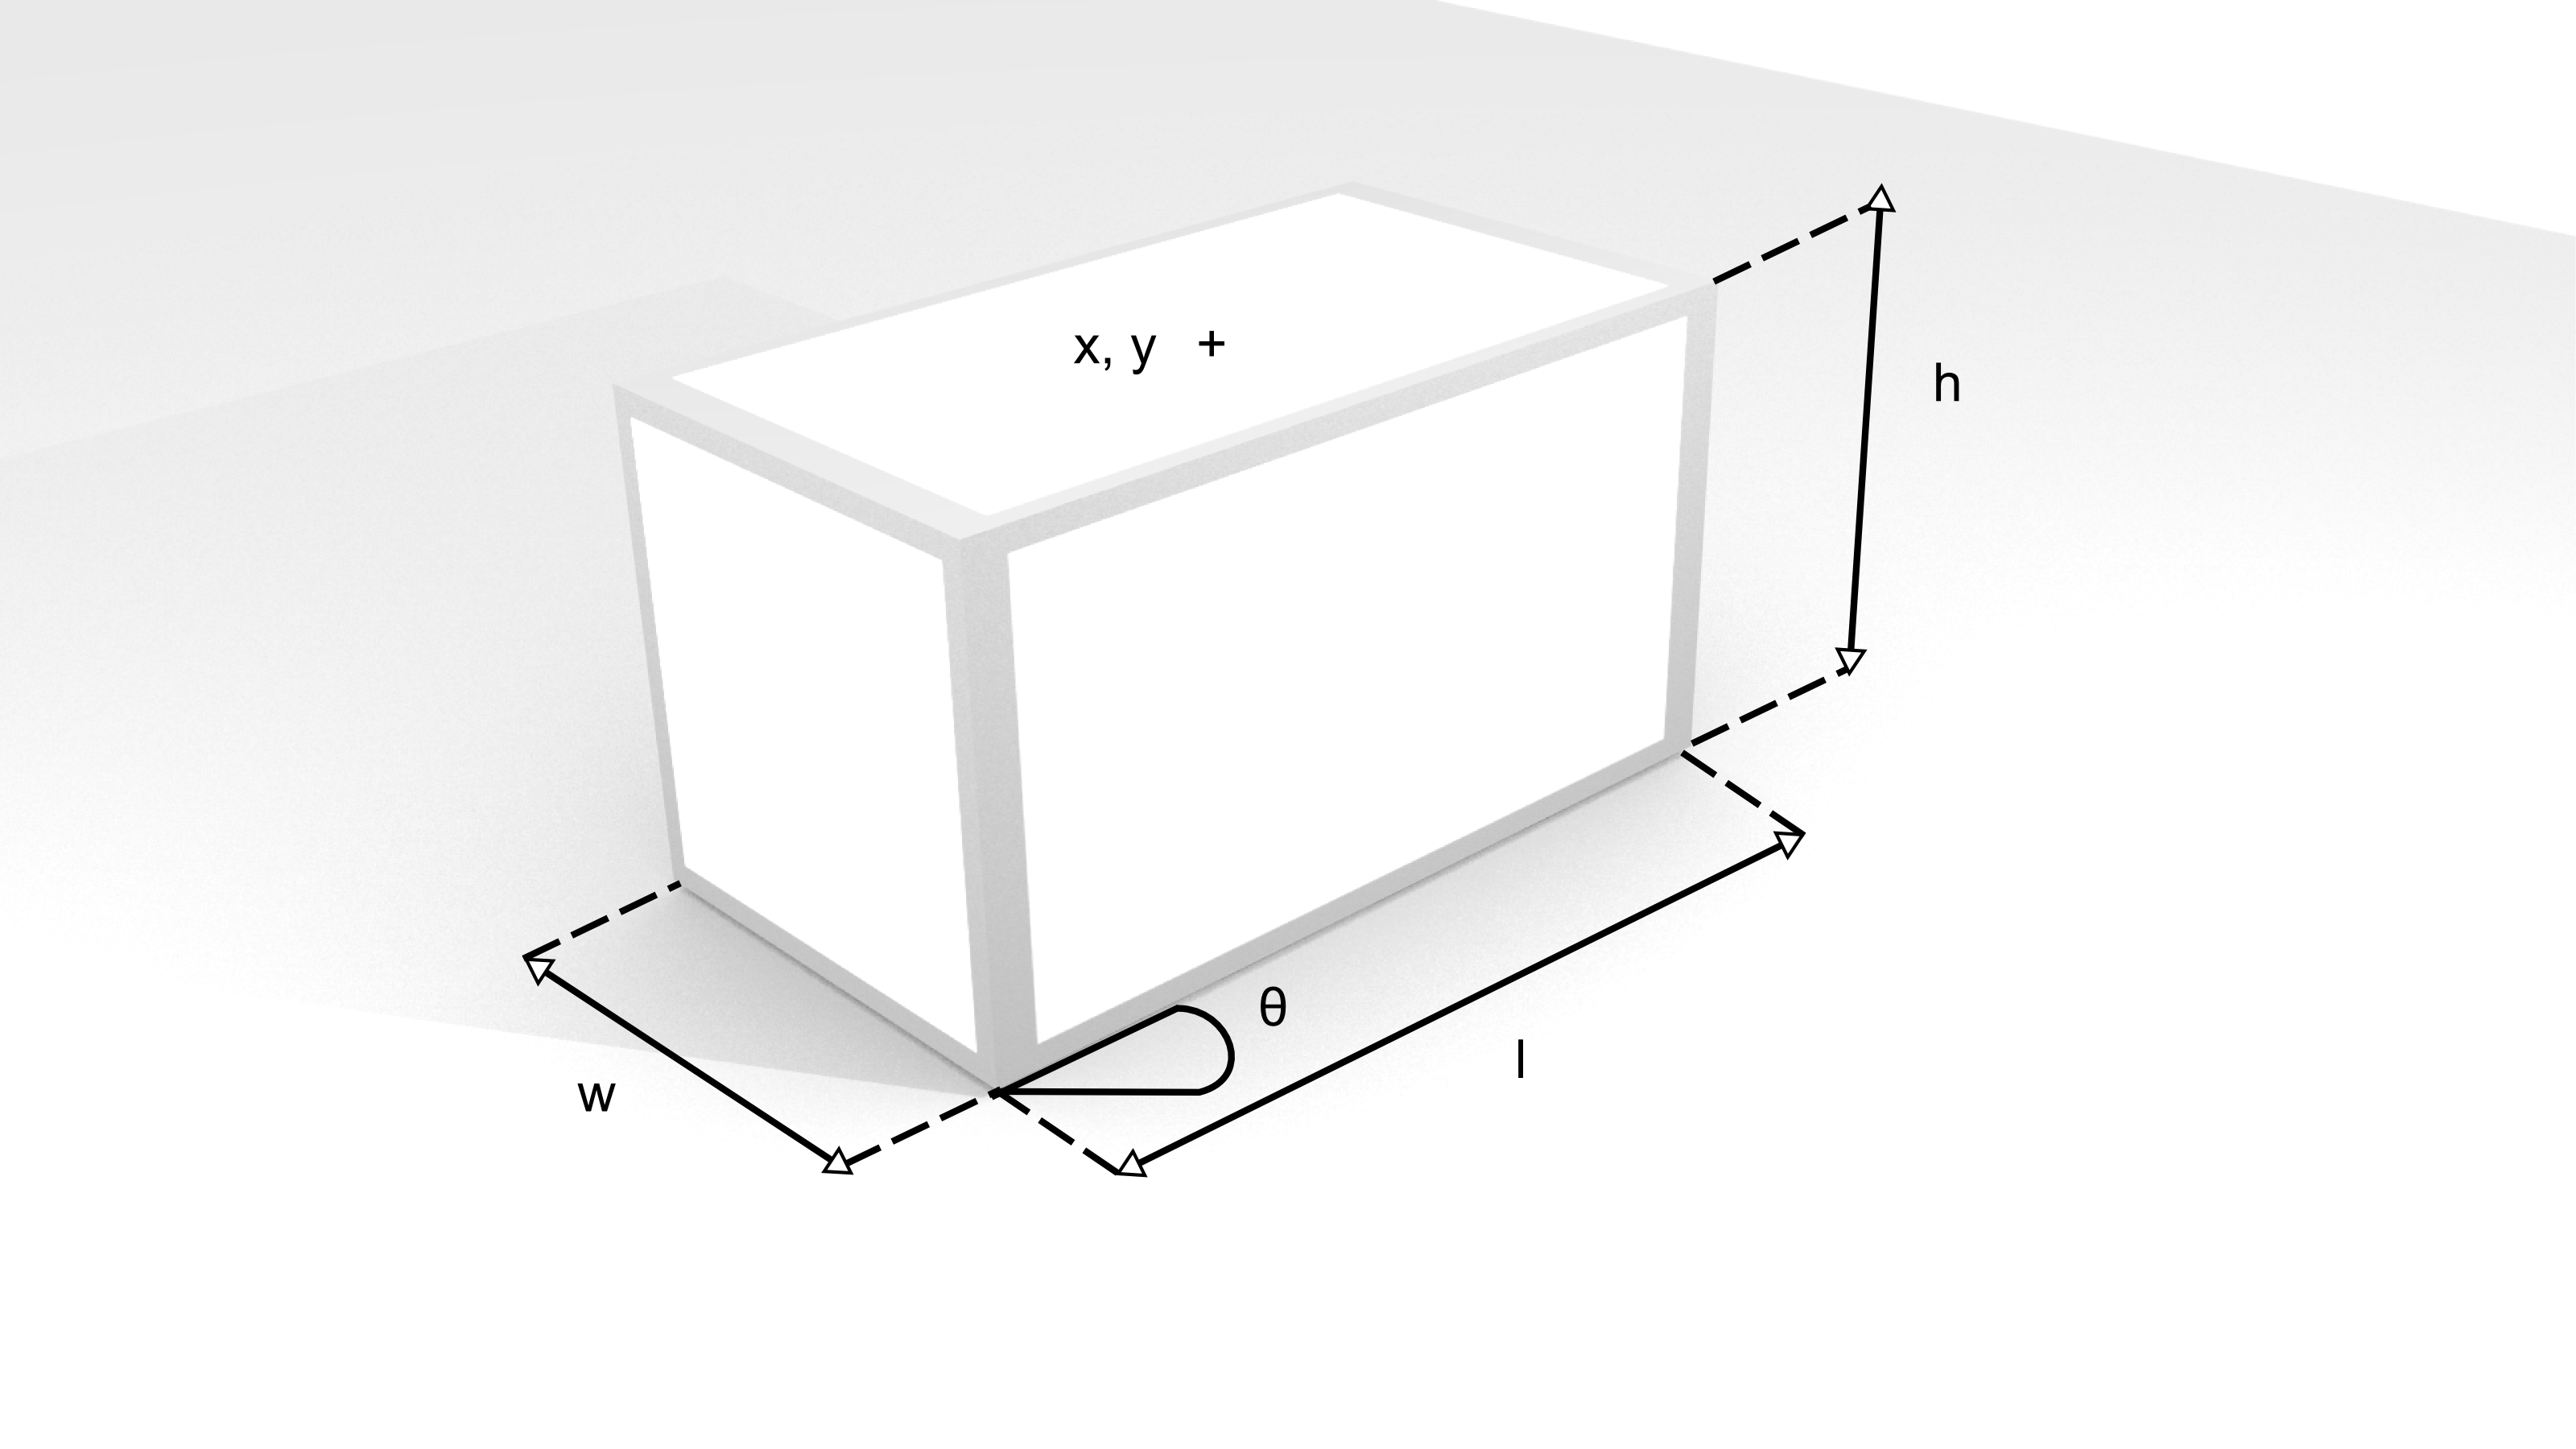
\includegraphics[width=\textwidth]{boiteFin.png}
\end{column}
\end{columns}
\begin{itemize}
\item Énergie~: $\mu = \mu_{unaire} + 2 \times \mu_{binaire}$
\begin{itemize}
\item $\tilde \mu_{unaire}(b \in \mathcal{B})=\alpha_{0} - volume(b)$ avec $\alpha_{0} \in \Re^{+*}$ ;
\item $\tilde \mu_{binaire}(b \in \mathcal{B}, b' \in \mathcal{B})) = volume(b \cap b')$.
\end{itemize}
\item Contraintes~:  $\mathcal{PLU}$, implémentation par rejet (taux d'acceptation à 0)
\end{itemize}


\end{frame}

\begin{frame}
\frametitle{Simplu3D}
\emph{R\'esultats:}
 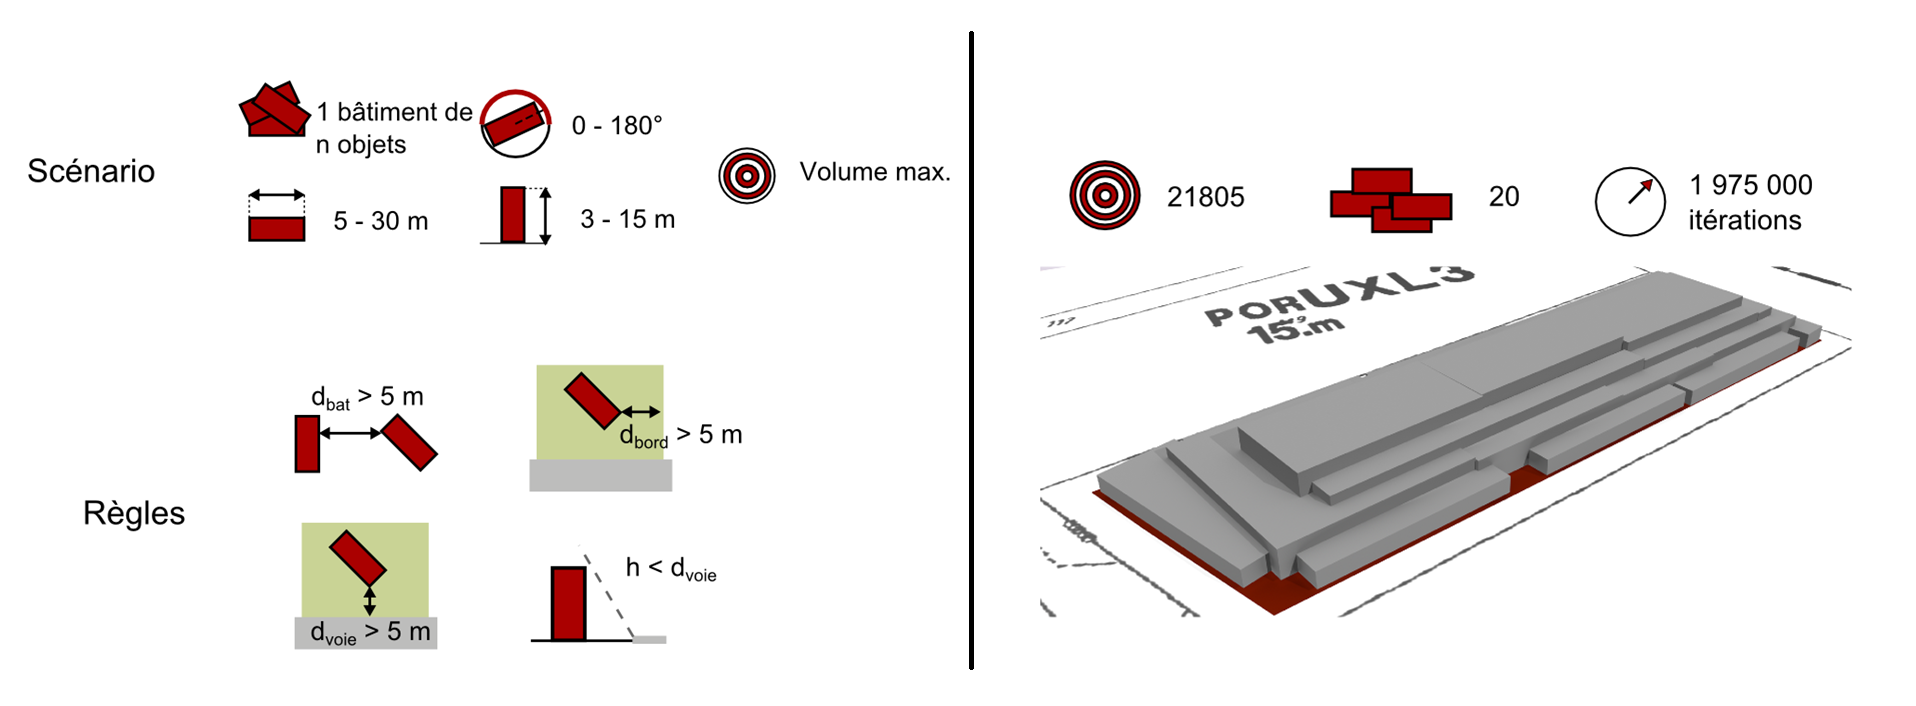
\includegraphics[width=\textwidth]{simplu3D1.png}
\end{frame}

\begin{frame}
\frametitle{Simplu3D}
\emph{R\'esultats:}
 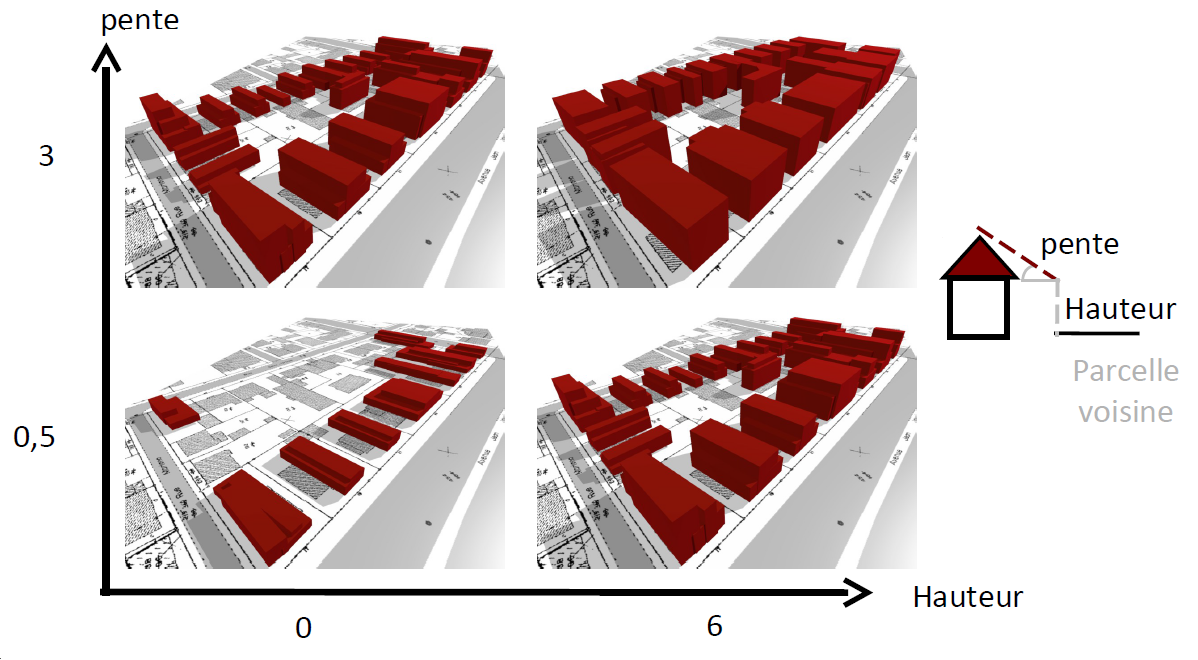
\includegraphics[width=\textwidth]{simplu3D2.png}
\end{frame}





\begin{frame}
\frametitle{Extraction des marquages aux sols}
\begin{center}
\begin{figure}[ht]
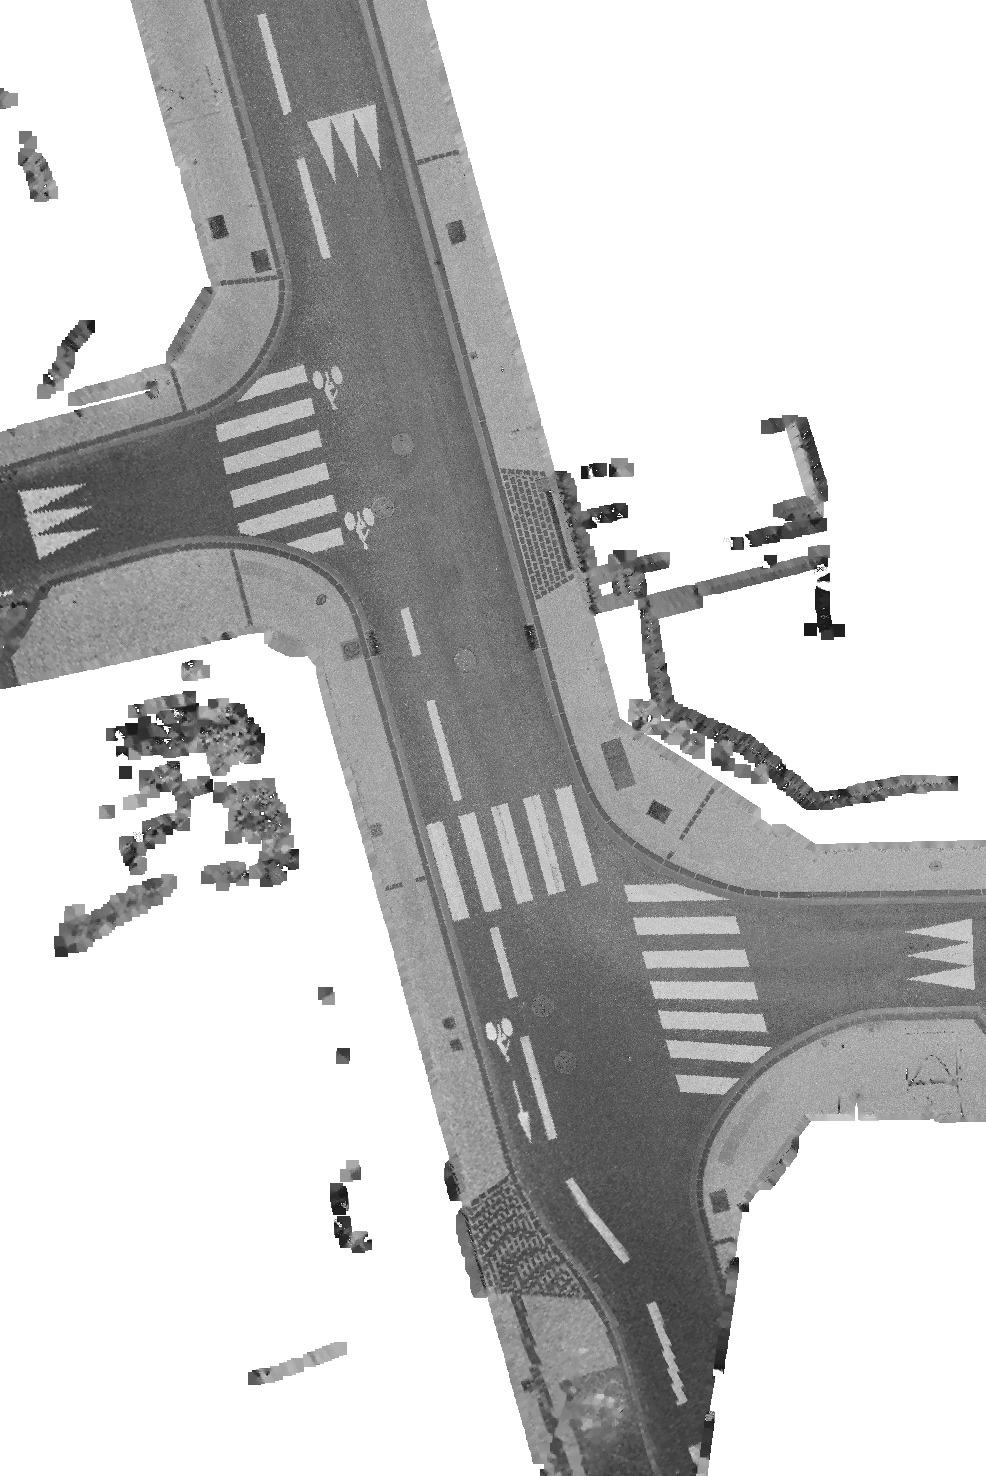
\includegraphics[angle = 90, width = .85\linewidth, scale = 0.7]{im_basis_crop_white}
\end{figure}
\begin{figure}[ht]

\includegraphics[scale = \patternscale]{patterns/1.jpg}\hspace*{\patternspace}

\includegraphics[scale = \patternscale]{patterns/2.jpg}\hspace*{\patternspace}

\includegraphics[scale = \patternscale]{patterns/3.jpg}\hspace*{\patternspace}

\includegraphics[scale = \patternscale]{patterns/4.jpg}\hspace*{\patternspace}

\includegraphics[scale = \patternscale]{patterns/5.jpg}\hspace*{\patternspace}

\includegraphics[scale = \patternscale]{patterns/6.jpg}\hspace*{\patternspace}

\includegraphics[scale = \patternscale]{patterns/7.jpg}
\end{figure}
\end{center}
\end{frame}

\begin{frame}
\frametitle{Extraction des marquages aux sols}
\emph{Le probl\`eme~:} 
\begin{itemize}
\item Détecter différents types de marquages sur une ortho-image.
\end{itemize}
\emph{Les concepts~:}
\begin{itemize}
\item MPP~:  $\mathcal{C} = \cup_{n}\mathcal{B}^n$\\
avec $\mathcal{B}=\{1...\vert \mathcal{L}\vert\}\times [0,W]\times[0,H]\times[-\pi,\pi]\times[\lambda-\epsilon,\lambda + \epsilon] \subset  \mathds{R}^{5}$
\item Noyaux~: Naissance/mort, translation, rotation, changement d'échelle, changement de type. 
\item Processus de référence~:
\begin{itemize}
\item Processus de poisson sur $n$
\item \color{red}{Data\&Model driven}
\end{itemize}
\item \'Energie~: $E = \sum_i E_1(x_i) + \sum_{i<j} E_2(x_i,x_j)$
\begin{itemize}
\item $E_1(x_i)=\alpha_{0} - E_{data}(x_i)$ avec $\alpha_{0}>0$ ;
\item $E_2(x_i,x_j) = \frac{(x_i \cap x_j)}{min(surface(x_i),surface(x_j)}$.
\end{itemize}
\end{itemize}
\end{frame}
%
\begin{frame}
\frametitle{Extraction des marquages aux sols}
\emph{R\'esultats~:}
\begin{center}
%\begin{figure}[ht]
%\animategraphics[scale=0.5, controls]{12}{}{1}{92}
%\end{figure}
%\movie[autostart,poster,externalviewer=/usr/bin/mplayer]{}{./images/video/animated.avi}
%\href{run:/usr/bin/mplayer -fs ./images/video/animated.avi}{Go}
\includemedia[addresource=animated.avi]{}{animated.avi}
\end{center}
\end{frame}


\begin{frame}{Model-driven perturbation kernels}
We look for type and geometric  modifications that may be applied to an object, to yield a new object providing similar reconstructed image.

%\begin{itemize}
%\item Simultaneous modification of all parameters $(\ell_i,x_i,y_i,\theta_i,\lambda_i)$.
%\item Distribution of such modifications is predicted using the collection of road-marking templates
%\begin{itemize}
 For $X_i=(\ell_i,0,0,0,1)$ and another object $X_j=(\ell_j,x_j,y_j,\theta_j,\lambda_j)$:

\begin{eqnarray}
\nonumber &&\ell_j\ \in \lbrace 1 \dots |\mathcal{L}|\rbrace\\
\nonumber &&(x_j,y_j) \in [-\Delta_x,\delta_x,\Delta_x]\times [-\Delta_y,\delta_y,\Delta_y]\\
\nonumber &&\theta_i \in [-\pi,\delta_\theta,\pi]\\
\nonumber &&\lambda_i \in [1-\Delta_\lambda,\delta_\lambda,1+\Delta_\lambda]\\
\nonumber && M_i \leftarrow ZMNC (I_{rec}(X_i),I_{rec}(X_j))
\end{eqnarray} 
%\end{itemize}
%\end{itemize}
The more a pair of objects $I_{rec}(X_i)$ and $I_{rec}(X_j)$ are similar the more corresponding perturbation is favoured to be tested. 
\end{frame}

\begin{frame}{Model-driven perturbation kernels: example 1}
\begin{itemize}
\item A $\texttt{BIKE}$ looks similar to a $y_j^*$-shifted $\pi$-rotated $\texttt{BIKE}$.
\item The model-driven perturbation kernel will encourage such modification to be tested.
\end{itemize}

\begin{figure}
\centering
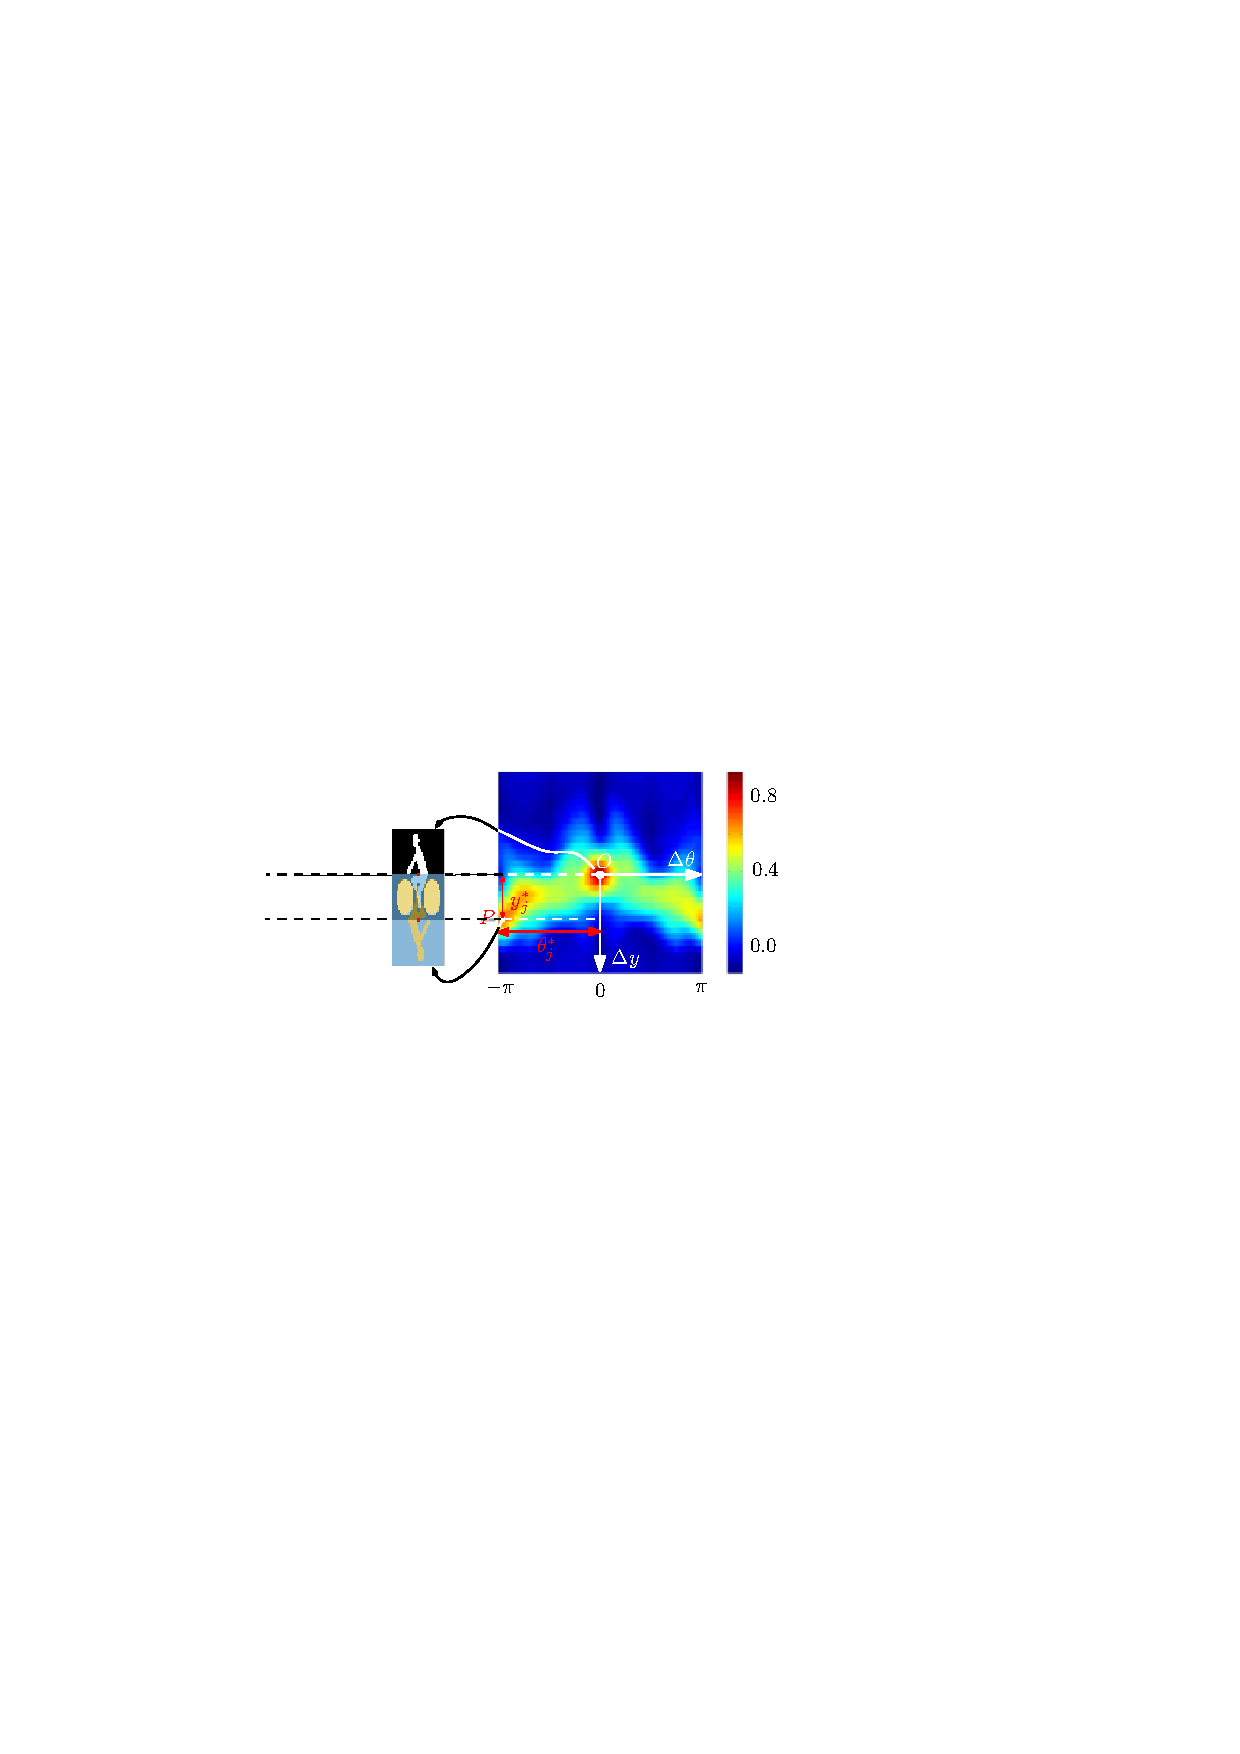
\includegraphics[width = 0.9\linewidth]{correlation_velo_velo}
\caption{Geometric transformation perturbation without type modification}
\end{figure}
\end{frame}

\begin{frame}{Model-driven perturbation kernels: example 2}
\begin{itemize}
\item A $\texttt{BIG ARROW}$  looks similar to a $y_j^*$-shifted $\texttt{TRIANGLE}$ 
 \item The model-driven perturbation kernel will encourage such geometric and type modification of to be tested.
\end{itemize}

\begin{figure}
\centering
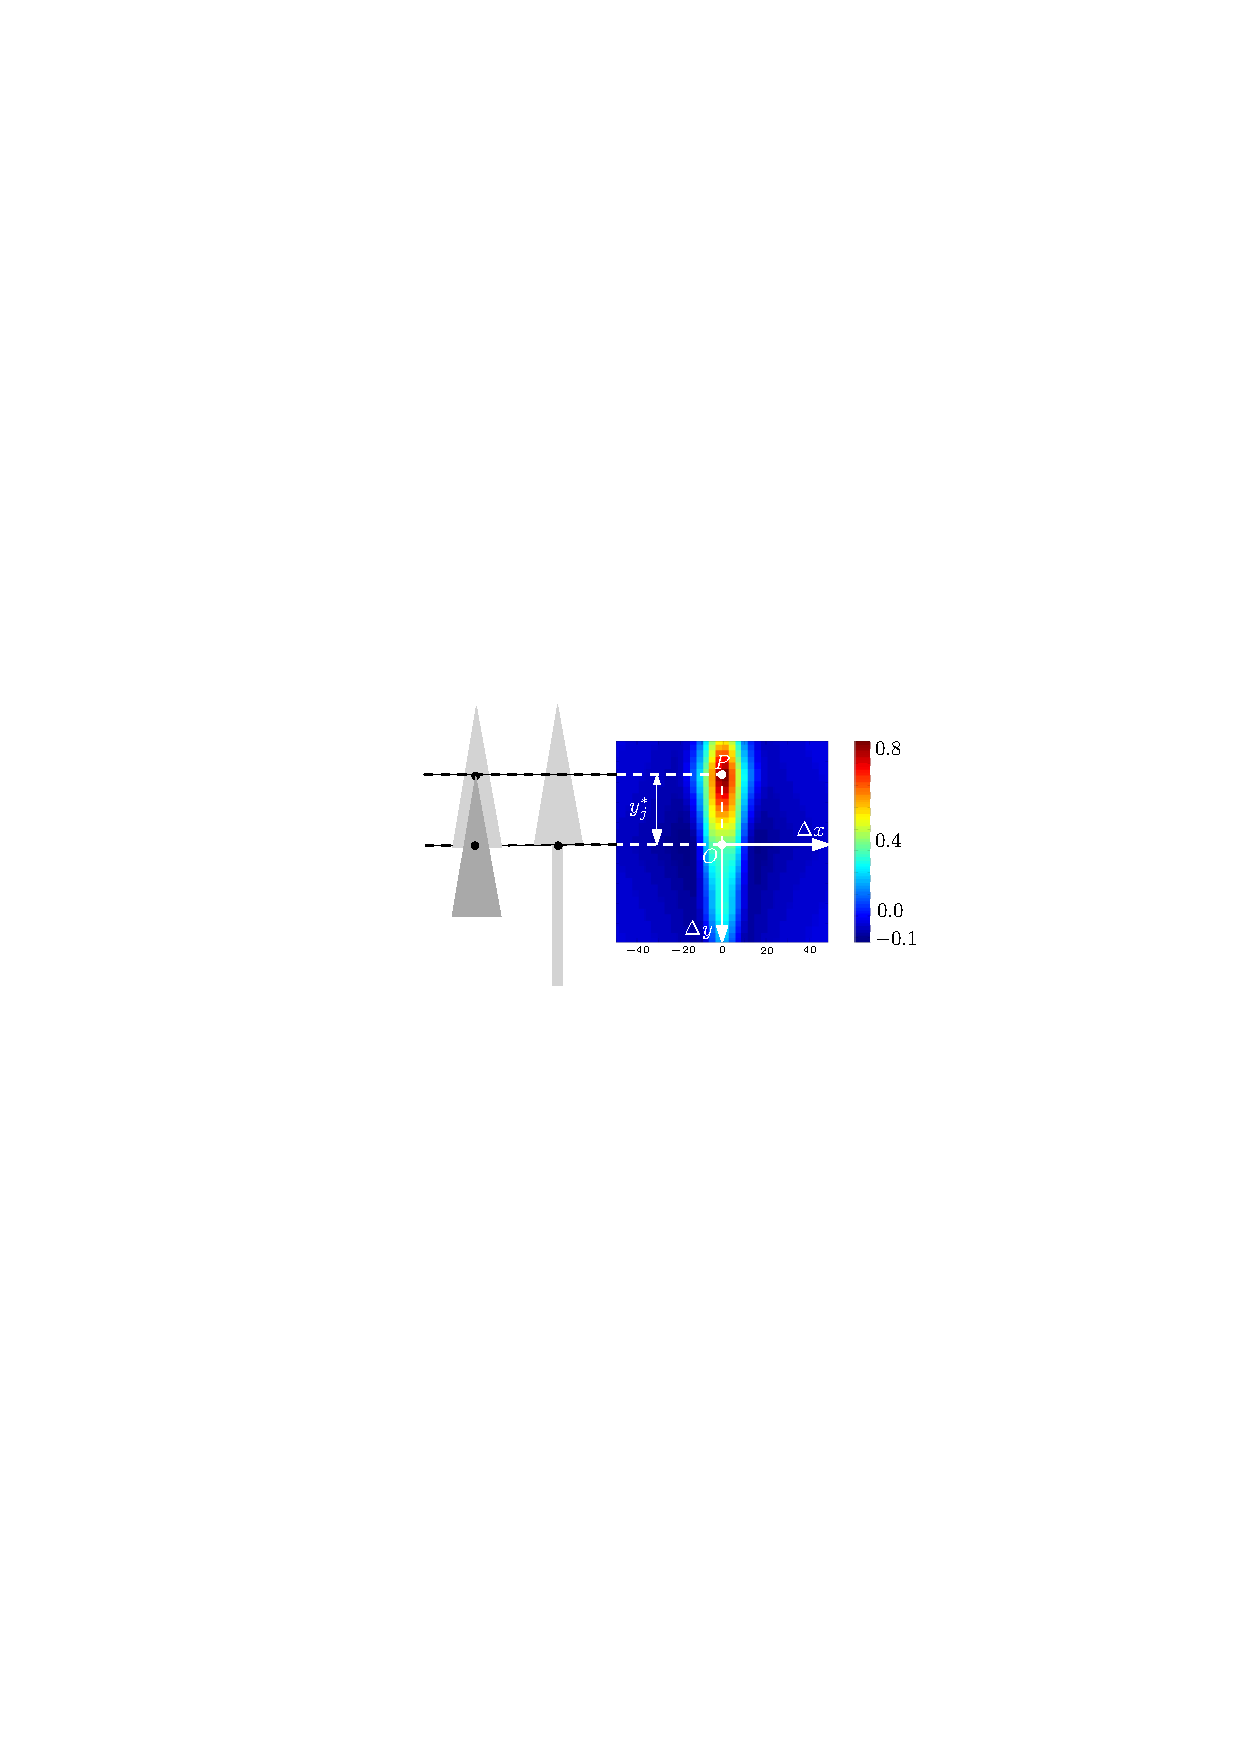
\includegraphics[width = 0.9\linewidth]{correlation_f_t}
\caption{Type modification together with geometric transformation.}
\end{figure}
\end{frame}

\begin{frame}
\frametitle{Autres applications}
\begin{itemize}
\item Symbologie C Rémy
\item JPB
\item multi objets...
\end{itemize}
\end{frame}


\section{Reproductibilité}
\begin{frame}
\frametitle{La \emph{libRJMCMC}}
Elle propose~:
\begin{itemize}
\item un \'echantillonneur RJMCMC
\item un recuit simul\'e (ou parallel tempering)
\item des exemples et des applications
\end{itemize}
Plusieurs impl\'ementations~:
\begin{itemize}
\item C++ \small[\url{http://github.com/IGNF/librjmcmc}]
\item Java \small[\url{http://github.com/IGNF/librjmcmc4j}]
\item Scala \small[\url{http://github.com/IGNF/librjmcmc4s}]
\end{itemize}
Le tout sous licence libre : CeCILL-B.
\end{frame}



\begin{frame}
\frametitle{Coal Mining}
Exemple de change point analysis de Green (1995).
\begin{itemize}
\item 
\item 
\item 
\end{itemize}
\end{frame}

\begin{frame}
\frametitle{Lamps}
Exemple de problème d'optimisation pour la programmation génétique d'Alberto Tonda (2010?).
\begin{itemize}
\item 
\item 
\item 
\end{itemize}
\end{frame}

\section{Conclusion}
\begin{frame}
\frametitle{Conclusion et perspectives}
\begin{itemize}
\item Recherche reproductible
\item $\Rightarrow$ Appel à Contribution ?
\end{itemize}
\emph{Nouvelles applications~:} 
\begin{itemize}
\item Maillage simplifié (espace de recherche des triangulations)
\item Appariement de données
\item Recalage
\item ...
\end{itemize}

\emph{Parallelisation et passage à l'échelle:} 
\begin{itemize}
\item Rien de spécifique au géospatial ni a l'espace ambient pour l'instant (cf Verdié)
\item Distributed tempering
\item Openmole
\end{itemize}

\end{frame}
\begin{frame}{RJMCMC + Recuit Simulé = Optimisation Stochastique}

\begin{block}{Recuit simulé}
La pdf cible $f_n(x)$ dépend d'une énergie $E(x)$ et d'une température $T_n$ :
\begin{itemize}
\item \textit{e.g.:} $f_n(x) = \frac{1}{Z}.e^\frac{-E(x)}{T_n}$
\end{itemize}
\end{block}

\begin{block}{Optimisation stochastique }
Avec $T_n\overset{n\rightarrow\infty}{\longrightarrow} 0$ (suffisament lentement), $f_n$ échantillonne le(s) \textbf{minimum global de $E$} 
\begin{itemize}
\item En pratique, schéma de décroissance géométrique $T_n=\alpha^n.T_0$
\end{itemize}
\end{block}

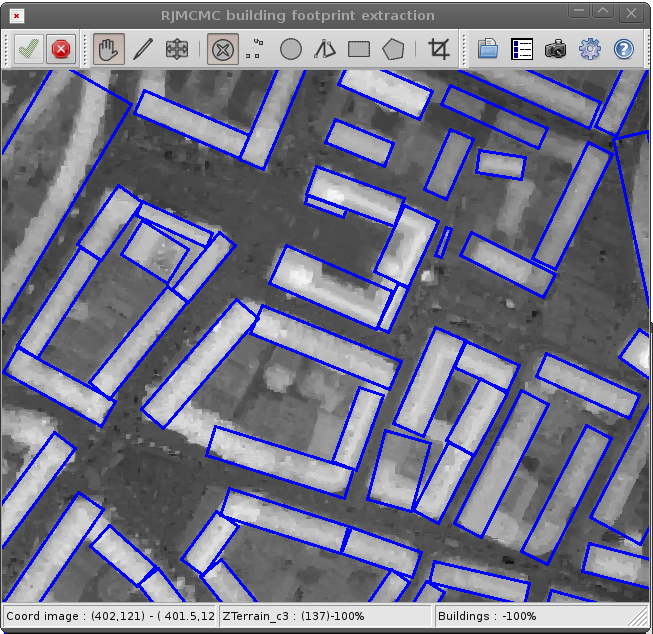
\includegraphics[height=2.8cm]{configuration}\hfill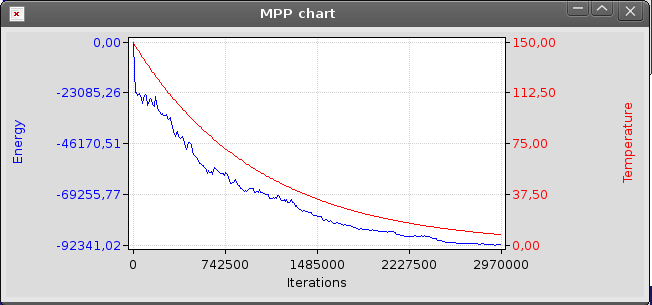
\includegraphics[height=2.8cm]{schedule}
\end{frame}

%%%%%%%%%%%%%%%%%%%%%%%%%%%%%%%%%%%%%%%%%%%%%%%%%%%%%%%%%%%%%%%%%%%%%%%%%%%%%%%%%%%%%%%%%%%%%%%%%%%%%%%%%
%%% SECTION
%%%%%%%%%%%%%%%%%%%%%%%%%%%%%%%%%%%%%%%%%%%%%%%%%%%%%%%%%%%%%%%%%%%%%%%%%%%%%%%%%%%%%%%%%%%%%%%%%%%%%%%%%
\section*{Library}

\begin{frame}[containsverbatim]{Library - Quickstart Code Sample}
\tiny
\begin{lstlisting}
// Objects are circle
typedef Circle_2<Simple_cartesian<double> >                     object;
// Objective function
typedef constant_energy<>                                       energy1;
typedef intersection_area_binary_energy<>                       area;
typedef multiplies_energy<constant_energy<>,area>               energy2;
typedef graph_configuration<object, energy1, energy2>           configuration;
// Reference process
typedef poisson_distribution                                    distribution;
typedef uniform_birth<object>                                   uniform_birth;
typedef direct_sampler<distribution,uniform_birth>              reference_process;
// RJMCMC sampler
typedef metropolis_acceptance                                   acceptance;
typedef result_of_make_uniform_birth_death_kernel<object>::type kernel;
typedef rjmcmc::sampler<reference_process,acceptance, kernel>   sampler;
\end{lstlisting}
\begin{lstlisting}
// Reference process
distribution dpoisson(200);
uniform_birth birth( Circle_2(Point_2(0,0),0.02), Circle_2(Point_2(1,1),0.1) );
reference_process reference_pdf( dpoisson, birth );
// Empty configuration linked with the minimized energy
configuration c(-1, 10000.*area());
// Visitors
ostream_visitor osvisitor; tex_visitor texvisitor("quickstart_");
composite_visitor<ostream_visitor,tex_visitor>  visitor(osvisitor,texvisitor);
// Simulated Annealing
sampler samp( reference_pdf, acceptance(), make_uniform_birth_death_kernel(birth,
geometric_schedule<double> sch(200.,0.999999);                         0.5,0.5));
max_iteration_end_test     end(10000001);
optimize(c,samp,sch,end,visitor);
\end{lstlisting}

\end{frame}

\begin{frame}{Librairie}

\begin{block}{Sortie du code de la diapo précédente (356 objets, 11s)}
   \begin{minipage}[c]{.3\linewidth}
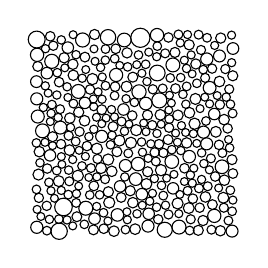
\begin{tikzpicture}[scale=2.5]
\draw (0.443809,0.618626) circle (0.0292179);
\draw (0.980845,0.721945) circle (0.0231037);
\draw (0.792965,0.244316) circle (0.0208813);
\draw (0.653285,0.00750491) circle (0.0382875);
\draw (0.753014,0.252608) circle (0.0200616);
\draw (0.522584,0.707994) circle (0.0362092);
\draw (0.187824,0.99845) circle (0.0202837);
\draw (0.377824,0.439447) circle (0.0218733);
\draw (0.86276,0.560115) circle (0.0220988);
\draw (0.285931,0.773061) circle (0.0286654);
\draw (0.185809,0.364137) circle (0.0206749);
\draw (0.115053,0.254509) circle (0.0277328);
\draw (0.0717843,0.990404) circle (0.0243194);
\draw (0.52941,0.982707) circle (0.0487341);
\draw (0.352442,0.739493) circle (0.0222885);
\draw (0.165154,0.48572) circle (0.023554);
\draw (0.399038,0.876828) circle (0.0221946);
\draw (0.937748,0.981378) circle (0.0261185);
\draw (0.53686,0.18801) circle (0.0296735);
\draw (0.0564095,0.318612) circle (0.0241013);
\draw (0.904832,0.595531) circle (0.0290595);
\draw (0.214438,0.710303) circle (0.0354649);
\draw (0.461732,0.906324) circle (0.0261391);
\draw (0.517991,0.341472) circle (0.0344815);
\draw (0.126409,0.442923) circle (0.0239751);
\draw (0.299219,0.863452) circle (0.020126);
\draw (0.624302,0.442775) circle (0.0238299);
\draw (0.220495,0.505962) circle (0.02371);
\draw (0.720097,0.589341) circle (0.0267962);
\draw (0.0759988,0.598863) circle (0.0213638);
\draw (0.511153,0.84638) circle (0.0203918);
\draw (0.00272553,0.973979) circle (0.0429755);
\draw (0.33342,0.546394) circle (0.0203132);
\draw (0.211793,0.281776) circle (0.0285741);
\draw (0.00482571,0.896239) circle (0.03386);
\draw (0.929005,0.438946) circle (0.0242491);
\draw (0.880052,0.312034) circle (0.0207014);
\draw (0.366835,0.200316) circle (0.0262166);
\draw (0.365231,0.985541) circle (0.0391696);
\draw (0.122679,0.526765) circle (0.0330486);
\draw (0.459346,0.734601) circle (0.0277789);
\draw (0.306461,0.579172) circle (0.0205404);
\draw (0.0321889,0.51013) circle (0.0352688);
\draw (0.796044,0.165545) circle (0.0243245);
\draw (0.10507,0.692125) circle (0.0213012);
\draw (0.560098,0.240329) circle (0.0277703);
\draw (0.823744,0.00469203) circle (0.0256373);
\draw (0.0705512,0.385449) circle (0.0289954);
\draw (0.434234,0.557485) circle (0.0230167);
\draw (0.769239,0.205692) circle (0.0224937);
\draw (0.694715,0.844929) circle (0.0353848);
\draw (0.986432,0.208489) circle (0.0223057);
\draw (0.0717077,0.557128) circle (0.0202079);
\draw (0.571694,0.0888105) circle (0.0291364);
\draw (0.705026,0.908419) circle (0.025616);
\draw (0.426445,0.228069) circle (0.0291443);
\draw (0.893889,0.826292) circle (0.023652);
\draw (0.519942,0.895479) circle (0.0219769);
\draw (0.695443,0.218061) circle (0.0290579);
\draw (0.185898,0.0271946) circle (0.020264);
\draw (0.866202,0.443998) circle (0.0305961);
\draw (0.620223,0.0607534) circle (0.0239195);
\draw (0.508266,0.513731) circle (0.0284224);
\draw (0.950998,0.170241) circle (0.0277481);
\draw (0.296601,0.999559) circle (0.0259001);
\draw (0.188602,0.792484) circle (0.0265044);
\draw (0.335696,0.783517) circle (0.0208919);
\draw (0.912911,0.505126) circle (0.0274933);
\draw (0.558099,0.505734) circle (0.0204458);
\draw (0.127801,0.379283) circle (0.0204103);
\draw (0.800811,0.320049) circle (0.0207424);
\draw (0.655295,0.903703) circle (0.022816);
\draw (0.18664,0.848401) circle (0.0264606);
\draw (0.0194901,0.34787) circle (0.0214911);
\draw (0.576974,0.152736) circle (0.0210092);
\draw (0.832695,0.622952) circle (0.0202907);
\draw (0.944088,0.327544) circle (0.0347298);
\draw (0.734219,0.780557) circle (0.0217847);
\draw (0.165459,0.310676) circle (0.0217213);
\draw (0.687169,0.651013) circle (0.020068);
\draw (0.858499,0.779237) circle (0.023134);
\draw (0.406245,0.79393) circle (0.033508);
\draw (0.850198,0.503627) circle (0.0309252);
\draw (0.200802,0.45643) circle (0.022556);
\draw (0.292977,0.51814) circle (0.0211677);
\draw (0.00825147,0.582868) circle (0.0330771);
\draw (0.615441,0.940513) circle (0.0220169);
\draw (0.138844,0.123263) circle (0.0447423);
\draw (0.689289,0.414304) circle (0.0220355);
\draw (0.244737,0.0350895) circle (0.0218894);
\draw (0.333108,0.481997) circle (0.0309482);
\draw (0.972657,0.522469) circle (0.0241374);
\draw (0.0611037,0.701722) circle (0.0203803);
\draw (0.390553,0.531709) circle (0.0252537);
\draw (0.0546349,0.803259) circle (0.0295129);
\draw (0.350375,0.264198) circle (0.0225804);
\draw (0.825152,0.998637) circle (0.0227098);
\draw (0.352435,0.925687) circle (0.0223487);
\draw (0.856572,0.681061) circle (0.020128);
\draw (0.296594,0.0639354) circle (0.0294569);
\draw (0.612057,0.122411) circle (0.0216395);
\draw (0.566528,0.302164) circle (0.0257043);
\draw (0.760544,0.645515) circle (0.0213781);
\draw (0.0674381,0.0605282) circle (0.0213343);
\draw (0.785135,0.0609234) circle (0.0232363);
\draw (0.775289,0.117767) circle (0.0275971);
\draw (0.0448732,0.451861) circle (0.0204394);
\draw (0.491361,0.145247) circle (0.0267407);
\draw (0.412866,0.0830847) circle (0.0319107);
\draw (0.10744,0.805483) circle (0.0218623);
\draw (0.512565,0.088737) circle (0.0215124);
\draw (0.478081,0.205578) circle (0.0258292);
\draw (0.232807,0.331691) circle (0.0219906);
\draw (0.956182,0.259402) circle (0.0268689);
\draw (0.293799,0.926427) circle (0.0202082);
\draw (0.540236,0.401364) circle (0.0211239);
\draw (0.464752,0.835182) circle (0.0219182);
\draw (0.142069,0.881129) circle (0.0261524);
\draw (0.809093,0.672163) circle (0.0279428);
\draw (0.671958,0.984419) circle (0.0240905);
\draw (0.121682,0.620229) circle (0.0227116);
\draw (0.334655,0.670833) circle (0.0211902);
\draw (0.689113,0.354155) circle (0.0348109);
\draw (0.600545,0.267492) circle (0.0211292);
\draw (0.615222,0.804024) circle (0.0400143);
\draw (0.00310835,0.672625) circle (0.0307075);
\draw (0.0138336,0.169717) circle (0.0237107);
\draw (0.977321,0.465969) circle (0.0202883);
\draw (0.0118196,0.288109) circle (0.028125);
\draw (0.308495,0.419589) circle (0.0281561);
\draw (0.502753,0.0106956) circle (0.0271678);
\draw (0.614107,0.996349) circle (0.0339696);
\draw (0.992684,0.996312) circle (0.0206754);
\draw (0.718571,0.141255) circle (0.0281938);
\draw (0.982912,0.423708) circle (0.0217355);
\draw (0.127691,0.972041) circle (0.0216054);
\draw (0.759184,0.50181) circle (0.0201619);
\draw (0.631006,0.59154) circle (0.0271858);
\draw (0.753432,0.320085) circle (0.0243791);
\draw (0.612397,0.886755) circle (0.020924);
\draw (0.00155023,0.212821) circle (0.0219329);
\draw (0.0014517,0.760088) circle (0.0298227);
\draw (0.840732,0.398352) circle (0.0218024);
\draw (0.395275,0.000548528) circle (0.0269492);
\draw (0.59275,0.721203) circle (0.0236018);
\draw (0.919666,0.689476) circle (0.020174);
\draw (0.866926,0.874969) circle (0.0310969);
\draw (0.840449,0.263228) circle (0.0210549);
\draw (0.0870518,0.942448) circle (0.023657);
\draw (0.70014,0.289122) circle (0.0202212);
\draw (0.498972,0.654748) circle (0.0218913);
\draw (0.505804,0.264939) circle (0.0323221);
\draw (0.273692,0.720116) circle (0.0241386);
\draw (0.777511,0.379037) circle (0.0319763);
\draw (0.278555,0.321133) circle (0.0226436);
\draw (0.252124,0.821519) circle (0.0201157);
\draw (0.745756,0.695522) circle (0.0217231);
\draw (0.0652556,0.24854) circle (0.0221059);
\draw (0.384235,0.304616) circle (0.0267744);
\draw (0.816013,0.446534) circle (0.0202295);
\draw (0.21608,0.604744) circle (0.026064);
\draw (0.993234,0.856464) circle (0.0208438);
\draw (0.246076,0.561379) circle (0.026974);
\draw (0.613834,0.496823) circle (0.0211355);
\draw (0.463189,0.0583573) circle (0.0206455);
\draw (0.247771,0.884749) circle (0.0248886);
\draw (0.365819,0.364296) circle (0.0285763);
\draw (0.25018,0.380457) circle (0.0204679);
\draw (0.602122,0.400636) circle (0.0239152);
\draw (0.206912,0.0738135) circle (0.0252047);
\draw (0.218398,0.411064) circle (0.020164);
\draw (0.787503,0.895868) circle (0.0206442);
\draw (0.931273,0.890529) circle (0.030404);
\draw (0.565639,0.590193) circle (0.0255942);
\draw (0.852017,0.343949) circle (0.0214424);
\draw (0.0834297,0.435054) circle (0.0202931);
\draw (0.995256,0.000870071) circle (0.0304106);
\draw (0.204591,0.190613) circle (0.0212955);
\draw (0.568227,0.0262726) circle (0.0306356);
\draw (0.994925,0.363823) circle (0.0254368);
\draw (0.847695,0.0545118) circle (0.0260636);
\draw (0.769125,0.999066) circle (0.0206809);
\draw (0.43183,0.171889) circle (0.0248953);
\draw (0.371242,0.145729) circle (0.0283954);
\draw (0.171048,0.574666) circle (0.0269296);
\draw (0.45383,0.333609) circle (0.0310474);
\draw (0.535564,0.453483) circle (0.0216197);
\draw (0.965592,0.681455) circle (0.0214735);
\draw (0.608126,0.354728) circle (0.0227256);
\draw (0.732054,0.956946) circle (0.0209142);
\draw (0.116903,0.000278889) circle (0.0415417);
\draw (0.311563,0.367512) circle (0.0234653);
\draw (0.563034,0.760702) circle (0.0210479);
\draw (0.589767,0.539033) circle (0.0236151);
\draw (0.764847,0.448887) circle (0.0266109);
\draw (0.292369,0.632719) circle (0.020659);
\draw (0.572131,0.910098) circle (0.0206241);
\draw (0.62577,0.664664) circle (0.0383829);
\draw (0.398353,0.688917) circle (0.0222085);
\draw (0.724764,0.0893672) circle (0.0204983);
\draw (0.48809,0.587809) circle (0.024357);
\draw (0.481512,0.449384) circle (0.0285828);
\draw (0.0800199,0.643462) circle (0.0222543);
\draw (0.456856,0.673266) circle (0.0211769);
\draw (0.267958,0.480581) circle (0.0213081);
\draw (0.97688,0.054258) circle (0.0223577);
\draw (0.252115,0.117073) circle (0.0354843);
\draw (0.0536247,0.129167) circle (0.0238104);
\draw (0.0033026,0.0202505) circle (0.0309246);
\draw (0.931043,0.760617) circle (0.0271409);
\draw (0.634139,0.31044) circle (0.0287956);
\draw (0.556818,0.648715) circle (0.032262);
\draw (0.642725,0.72527) circle (0.0227847);
\draw (0.777152,0.947294) circle (0.0261208);
\draw (0.0161774,0.404207) circle (0.0267271);
\draw (0.410398,0.40383) circle (0.025332);
\draw (0.34323,0.0128433) circle (0.0244176);
\draw (0.45378,0.0082986) circle (0.0220393);
\draw (0.56881,0.370492) circle (0.0209217);
\draw (0.34225,0.0939826) circle (0.0221373);
\draw (0.556498,0.84808) circle (0.0221012);
\draw (0.169525,0.412227) circle (0.0273046);
\draw (0.189313,0.648778) circle (0.0224512);
\draw (0.329288,0.320804) circle (0.0280476);
\draw (0.645799,0.181125) circle (0.0224836);
\draw (0.717898,0.452224) circle (0.020776);
\draw (0.42321,0.460641) circle (0.0280452);
\draw (0.09287,0.167522) circle (0.0200213);
\draw (0.247454,0.652162) circle (0.0290471);
\draw (0.72576,0.0213535) circle (0.0354248);
\draw (0.999512,0.293342) circle (0.0246789);
\draw (0.448663,0.508356) circle (0.0215445);
\draw (0.961184,0.824032) circle (0.0234923);
\draw (0.67026,0.465321) circle (0.0251266);
\draw (0.0794508,0.863279) circle (0.0358608);
\draw (0.778559,0.602074) circle (0.027228);
\draw (0.168266,0.253633) circle (0.0228201);
\draw (0.00474523,0.111119) circle (0.0202743);
\draw (0.909532,0.278141) circle (0.0242442);
\draw (0.837624,0.920969) circle (0.0231897);
\draw (0.233984,0.777359) circle (0.0211409);
\draw (0.0833622,0.480369) circle (0.0255698);
\draw (0.906917,0.944036) circle (0.0205999);
\draw (0.447543,0.971627) circle (0.0349402);
\draw (0.927116,0.219772) circle (0.0201828);
\draw (0.258132,0.432855) circle (0.0241735);
\draw (0.792676,0.799584) circle (0.0200526);
\draw (0.145445,0.830121) circle (0.020125);
\draw (0.868179,0.982846) circle (0.0222136);
\draw (0.830705,0.11975) circle (0.0239852);
\draw (0.738324,0.536721) circle (0.020884);
\draw (0.657377,0.132299) circle (0.0213238);
\draw (0.764629,0.735949) circle (0.0222657);
\draw (0.998922,0.789823) circle (0.0257177);
\draw (0.404343,0.926921) circle (0.024575);
\draw (0.811362,0.849758) circle (0.0260026);
\draw (0.681283,0.778818) circle (0.0219975);
\draw (0.468044,0.39582) circle (0.0225447);
\draw (0.267488,0.273512) circle (0.0201532);
\draw (0.933295,0.643538) circle (0.0241253);
\draw (0.816355,0.75165) circle (0.0220056);
\draw (0.953319,0.11957) circle (0.0231164);
\draw (0.327357,0.832169) circle (0.0214139);
\draw (0.999787,0.928329) circle (0.0297216);
\draw (0.307465,0.126142) circle (0.0208549);
\draw (0.364764,0.0521283) circle (0.0204944);
\draw (0.590956,0.192867) circle (0.0208735);
\draw (0.636971,0.232943) circle (0.0219041);
\draw (0.881234,0.72861) circle (0.0325154);
\draw (0.450305,0.275863) circle (0.0214568);
\draw (0.161281,0.679801) circle (0.0204488);
\draw (0.804703,0.546227) circle (0.0286299);
\draw (0.00818711,0.837511) circle (0.0252853);
\draw (0.23596,0.971678) circle (0.0358692);
\draw (0.0464883,0.73859) circle (0.0211186);
\draw (0.293052,0.23038) circle (0.0247694);
\draw (0.987248,0.645312) circle (0.0218868);
\draw (0.127527,0.207499) circle (0.0209702);
\draw (0.202684,0.896839) circle (0.021477);
\draw (0.382861,0.618277) circle (0.0211115);
\draw (0.291156,0.00717197) circle (0.0252922);
\draw (0.675128,0.52604) circle (0.0237508);
\draw (0.995701,0.101558) circle (0.0221945);
\draw (0.735089,0.409749) circle (0.0213621);
\draw (0.539115,0.132037) circle (0.0206375);
\draw (0.160855,0.932925) circle (0.0292071);
\draw (0.157126,0.73401) circle (0.0212859);
\draw (0.904932,0.0782684) circle (0.0336637);
\draw (0.707917,0.72534) circle (0.0243223);
\draw (0.827224,0.218084) circle (0.022773);
\draw (0.88781,0.370226) circle (0.0228282);
\draw (0.116667,0.75751) circle (0.0245096);
\draw (0.351343,0.869368) circle (0.0214762);
\draw (0.895452,0.135542) circle (0.0249737);
\draw (0.881108,0.647211) circle (0.0205762);
\draw (0.859926,0.174252) circle (0.0270138);
\draw (0.0545112,0.00311648) circle (0.0221782);
\draw (0.752663,0.868876) circle (0.02057);
\draw (0.0240798,0.075086) circle (0.0200937);
\draw (0.871579,0.228535) circle (0.0227587);
\draw (0.401121,0.734487) circle (0.0247006);
\draw (0.0753809,0.205643) circle (0.0207504);
\draw (0.537027,0.802626) circle (0.0207794);
\draw (0.946191,0.397482) circle (0.0226392);
\draw (0.333247,0.617446) circle (0.0252001);
\draw (0.491073,0.782975) circle (0.0254484);
\draw (0.662863,0.269678) circle (0.0200213);
\draw (0.672224,0.0852496) circle (0.0230371);
\draw (0.272371,0.18422) circle (0.021918);
\draw (0.935953,0.0025299) circle (0.0262124);
\draw (0.708514,0.498804) circle (0.0202648);
\draw (0.461002,0.0990901) circle (0.0202524);
\draw (0.104708,0.308252) circle (0.0220721);
\draw (0.673785,0.615563) circle (0.0200387);
\draw (0.21616,0.229459) circle (0.0200086);
\draw (0.163276,0.186157) circle (0.0223047);
\draw (0.997968,0.598587) circle (0.0226117);
\draw (0.156839,0.0575507) circle (0.0210897);
\draw (0.582452,0.444252) circle (0.0207856);
\draw (0.31452,0.708051) circle (0.0206858);
\draw (0.0365467,0.62864) circle (0.0211464);
\draw (0.00120442,0.448866) circle (0.0218908);
\draw (0.111689,0.5778) circle (0.0213952);
\draw (0.32251,0.185011) circle (0.0217296);
\draw (0.890507,0.00802998) circle (0.0227726);
\draw (0.676538,0.569855) circle (0.0226312);
\draw (0.308266,0.27649) circle (0.0206296);
\draw (0.954701,0.567115) circle (0.0268464);
\draw (0.798757,0.495734) circle (0.020882);
\draw (0.397925,0.5808) circle (0.0205261);
\draw (0.130769,0.339936) circle (0.02004);
\draw (0.677448,0.691059) circle (0.0201691);
\draw (0.764101,0.827035) circle (0.0214542);
\draw (0.72291,0.999798) circle (0.0226039);
\draw (0.646191,0.398069) circle (0.0235613);
\draw (0.999317,0.158311) circle (0.0207291);
\draw (0.203343,0.144114) circle (0.0225585);
\draw (0.783638,0.28584) circle (0.0215425);
\draw (0.546123,0.549792) circle (0.0200737);
\draw (0.290778,0.67192) circle (0.0206721);
\draw (0.0472435,0.927208) circle (0.0209998);
\draw (0.729921,0.187195) circle (0.0202941);
\draw (0.634954,0.543719) circle (0.0202838);
\draw (0.174578,0.527675) circle (0.0211636);
\draw (0.424734,0.842665) circle (0.0200037);
\draw (0.471422,0.54393) circle (0.0200069);
\draw (0.779876,0.00383296) circle (0.0223911);
\draw (0.848705,0.821073) circle (0.0219498);
\draw (0.385626,0.487465) circle (0.021662);
\draw (0.115756,0.0616407) circle (0.0221326);
\draw (0.355329,0.574961) circle (0.0202238);
\end{tikzpicture}

   \end{minipage}
   \begin{minipage}[c]{.65\linewidth}
\setlength{\tabcolsep}{2pt}
\renewcommand\arraystretch{0.5}\scalebox{.4}{
\begin{tabular}{rrrrrrrrrrrr}
\tiny Iteration & Objects & Pkernel & Akernel & Pkernel & Akernel & Accept & Time(ms) & Temp & U\_1 & U\_2 & U\\
1000000 & 3 & 50.0251 & 6.91633 & 49.9749 & 6.92748 & 6.9219 & 250 & 73.5759 & -3 & -7.10543e-14 & -3 \\
2000000 & 4 & 50.0137 & 6.9189 & 49.9863 & 6.9251 & 6.922 & 250 & 27.0671 & -4 & -1.13687e-13 & -4\\
3000000 & 3 & 50.0744 & 6.70802 & 49.9256 & 6.73041 & 6.7192 & 260 & 9.95741 & -3 & -1.10134e-13 & -3 \\
4000000 & 4 & 49.9794 & 6.67955 & 50.0206 & 6.67465 & 6.6771 & 250 & 3.66312 & -4 & -1.04805e-13 & -4 \\
5000000 & 5 & 50.0122 & 6.64158 & 49.9878 & 6.64542 & 6.6435 & 270 & 1.34759 & -5 & -1.04805e-13 & -5\\
6000000 & 13 & 49.9979 & 6.48967 & 50.0021 & 6.48753 & 6.4886 & 290 & 0.495749 & -13 & -1.04583e-13 & -13\\
7000000 & 38 & 50.0199 & 5.25131 & 49.9801 & 5.25049 & 5.2509 & 430 & 0.182376 & -38 & -1.04305e-13 & -38\\
8000000 & 286 & 49.9434 & 1.48088 & 50.0566 & 1.42798 & 1.4544 & 1700 & 0.0670923 & -286 & 1.84745 & -284.153\\
9000000 & 333 & 49.9631 & 0.0140103 & 50.0369 & 0.00459661 & 0.0093 & 3490 & 0.0246819 & -333 & 8.72057 & -324.279\\
10000000 & 356 & 50.0272 & 0.00559696 & 49.9728 & 0.00100054 & 0.0033 & 3890 & 0.00907995 & -356 & 18.3511 & -337.649\\
\end{tabular}}
   \end{minipage}
\end{block}

\begin{block}{Librairie Open source C++}
\begin{itemize}
\item C++ générique : templates, cf  STL / CGAL / boost\\
\item Modulaire, Extensible
\begin{itemize}
 \item Modèles interchangeables pour les concepts orthogonaux: Schéma de température, énergies, noyaux...
 \item Visiteurs: console, latex, wx GUI, shapefile...
 \item Support pour du multi-objets
\end{itemize}
\end{itemize}
\end{block}

\end{frame}



\end{document}
